\section{Gallium Arsenide---Frequency-dependent spin Hall conductivity}
\label{sec30:GaAsSHC}

\begin{itemize}
	\item Outline: {\it Calculate the alternating current (ac) spin Hall conductivity
	of gallium arsenide considering spin-orbit coupling. 
	To gain a better understanding of this example, 
	it is suggested to read Ref.~\onlinecite{qiao-prb2018} for a detailed 
	description of the theory and Ch.~12.5 of the User Guide.}
\end{itemize}

\begin{itemize}
	\item[1-6] {\it Compute the MLWFs and compute the ac spin Hall conductivity.} 
\end{itemize}

\subsection*{ac spin Hall conductivity}

\begin{itemize}
	\item {\it The ac SHC of GaAs converges rather slowly with $k$-point sampling, and a $100 \times 100 \times 100$ kmesh does not yield a well-converged value.
	To get a converged SHC value, increase the density of kmesh and then compare the converged result with those obtained in Refs.~\onlinecite{qiao-prb2018}.}

	The file {\tt GaAs-shc-freqscan.dat} contains the calculated ac SHC. 
	The snippet below shows a calculated result with 
	$100\times100\times100$ kmesh, 
	a fixed smearing width of 0.05~eV and no scissors shift applied.

\begin{tcolorbox}[title=$100\times100\times100$ kmesh,sharp corners,boxrule=0.5pt]
{\small
\begin{verbatim}
#No.   Frequency(eV)   Re(sigma)((hbar/e)*S/cm)   Im(sigma)((hbar/e)*S/cm)
   1     0.000000    -0.68114601E+00    0.00000000E+00
...
 801     8.000000    -0.39471936E+01   -0.29928198E+02
\end{verbatim}
}
\end{tcolorbox}

The ac SHC is plotted as \Fig{fig30.1}.
\begin{figure}[htb!]
\centering
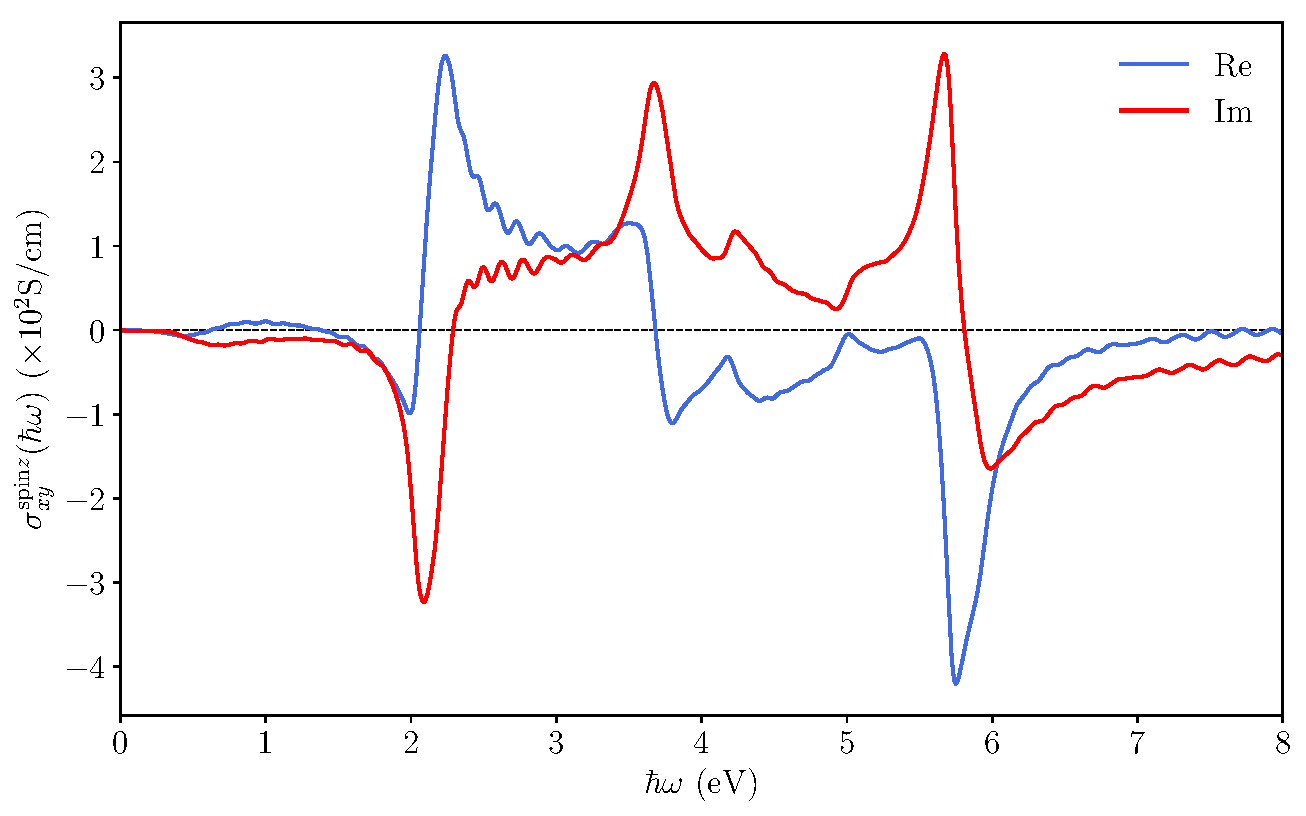
\includegraphics[width=.8\columnwidth]{figure/example30/gaas_freqscan_100kpt.pdf}
\caption{Frequency scan plot for GaAs ac SHC, using 
	a low kmesh of $100\times100\times100$.}
\label{fig30.1}
\end{figure}

\item If further increasing the density of kmesh to 
$250\times250\times250$, and using the adaptive smearing, 
a nice converged plot could be produced as \Fig{fig30.2}. 
Note that by using keywords \smallskip {\tt
	\begin{quote}
		shc\_bandshift = true
		
		shc\_bandshift\_firstband = 9
		
		shc\_bandshift\_energyshift = 1.117
\end{quote} }
a scissors shift of 1.117~eV is applied. 
\Fig{fig30.2} can be viewed as \Fig{fig30.1} translated by 
$\sim1$~eV along the horizontal axis. 
\begin{figure}[!htb]
\centering
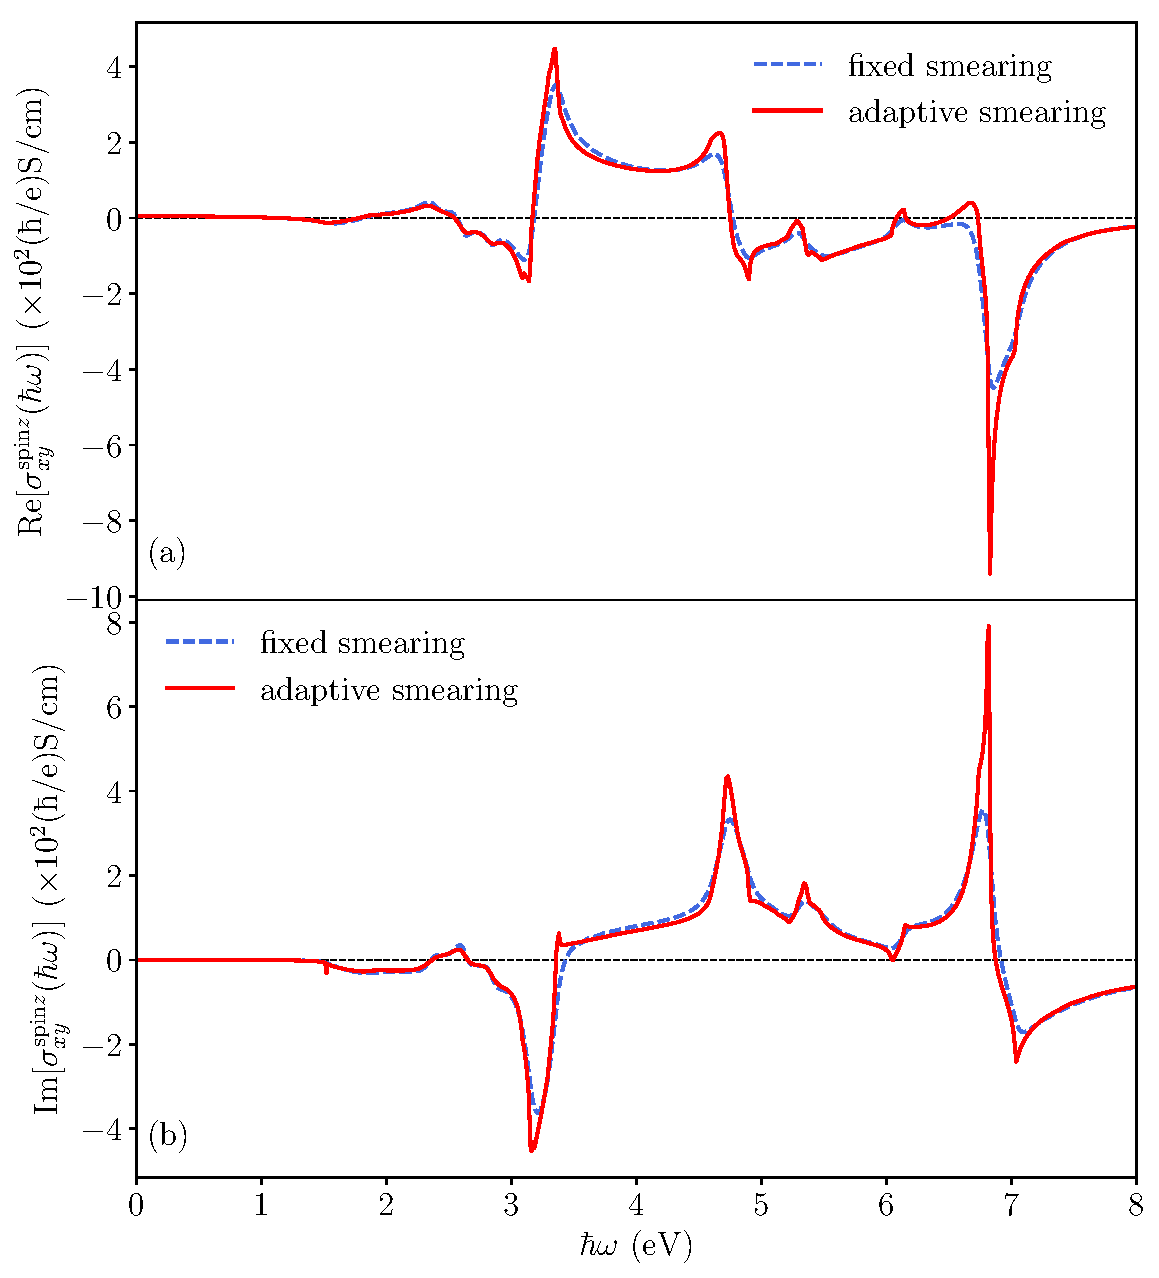
\includegraphics[width=0.8\columnwidth]{figure/example30/gaas_freqscan.pdf}
\caption{Frequency scan plots for GaAs ac SHC, using 
	a dense kmesh of $250\times250\times250$. 
Two kinds of smearing are compared.}
\label{fig30.2}
\end{figure}
\end{itemize}